\documentclass[compress, serif, onlymath, professionalfonts]{beamer}
\usepackage{amsmath, amssymb, amsfonts}%, mathrsfs}
\usepackage{subfigure,graphicx,enumerate}
\usepackage[]{algorithm2e}

\usepackage{times} 
\usepackage{bibentry}
\bibliographystyle{apalike}
%\usepackage{color}
%   5  \usepackage[colorlinks=true,linkcolor= blue]{hyperref}
%\usepackage{color}
%\usepackage{hyperref}
%5%5\usepackage[usenames,dvipsnames,svgnames,table]{xcolor}
\usepackage[square,sort,comma,numbers]{natbib}
\usepackage[utf8]{inputenc}
\usepackage[english]{babel}

    

    \usepackage{beamerthemesplit}

\usepackage{tikz}
\usetheme{Boadilla}
%\%usepackage{hyperref}
%\usetheme{Antibes}
\usecolortheme{beetle}
%\useoutertheme{split}
%\setbeamertemplate{navigation symbols}{}
\useoutertheme[footline=false]{tree}
\makeatletter
\setbeamertemplate{headline}
{%
    \begin{beamercolorbox}[wd=\paperwidth,colsep=1.5pt]{upper separation line head}
    \end{beamercolorbox}
    \begin{beamercolorbox}[wd=\paperwidth,ht=2.5ex,dp=1.125ex,%
      leftskip=.3cm,rightskip=.3cm plus1fil]{title in head/foot}
      \usebeamerfont{title in head/foot}\insertshorttitle
    \end{beamercolorbox}
    \begin{beamercolorbox}[wd=\paperwidth,ht=2.5ex,dp=1.125ex,%
      leftskip=.3cm,rightskip=.3cm plus1fil]{section in head/foot}
      \usebeamerfont{section in head/foot}%
      \ifbeamer@tree@showhooks
        \setbox\beamer@tempbox=\hbox{\insertsectionhead}%
        \ifdim\wd\beamer@tempbox>1pt%
          \hskip2pt\raise1.9pt\hbox{\vrule width0.4pt height1.875ex\vrule width 5pt height0.4pt}%
          \hskip1pt%
        \fi%
      \else%  
        \hskip6pt%
      \fi%
      \insertsectionhead
      \usebeamerfont{subsection in head/foot}%
      \ifbeamer@tree@showhooks
        \setbox\beamer@tempbox=\hbox{\insertsubsectionhead}%
        \ifdim\wd\beamer@tempbox>1pt%
          \ \raise1.9pt\hbox{\vrule width 5pt height0.4pt}%
          \hskip1pt%
        \fi%
      \else%  
        \hskip12pt%
      \fi%
      \insertsubsectionhead\hfill\insertframenumber/\inserttotalframenumber\hspace{0.5em}
    \end{beamercolorbox}
    \begin{beamercolorbox}[wd=\paperwidth,colsep=1.5pt]{lower separation line head}
    \end{beamercolorbox}
}
\makeatother

\makeatletter
\setbeamertemplate{footline}
{
  \leavevmode%
  \hbox{%
  \begin{beamercolorbox}[wd=.5\paperwidth,ht=2.25ex,dp=1ex,center]{author in head/foot}%
    \usebeamerfont{author in head/foot}\insertshortauthor%~~\beamer@ifempty{\insertshortinstitute}{}{(\insertshortinstitute)}
  \end{beamercolorbox}%
 
  \begin{beamercolorbox}[wd=.5\paperwidth,ht=2.25ex,dp=1ex,right]{date in head/foot}%
    \usebeamerfont{date in head/foot}\insertshortdate{}\hspace*{2em}
    %\insertframenumber{} / \inserttotalframenumber\hspace*{2ex} 
  \end{beamercolorbox}}%
  \vskip0pt%
}
\makeatother
%\useoutertheme[subsection=false]{tree}
%\usecolortheme{Seagull}
\definecolor{MidnightBlue}{rgb}{.3,.5,.85}
%\definecolor{darkchampagne}{rgb}{0.76, 0.7, 0.5}
%\definecolor{ballblue}{rgb}{0.13, 0.67, 0.8}
\setbeamercolor{palette primary}{fg=gray!30} %for setting font colour on topmost layer of header
\setbeamercolor{titlelike}{fg=black} %for setting font colour for title
\setbeamercolor{section in toc}{fg=black!80} %for setting font colour for Table of Contents
\setbeamercolor{block body}{bg=MidnightBlue!40} %for changing colour of block body. can specify colour for block title also, as below
\setbeamercolor{block title}{bg=MidnightBlue!80!black}
\setbeamercolor{background canvas}{bg=white} %or setting slide/frame background colour 
%\beamertemplateshadingbackground{white!25}{white!15} %for setting slide/frame background colour (in shades of 2 colours)

\setbeamercolor{bibliography entry author}{use=structure,fg=black} %for setting font colour of bibliographical entries
\setbeamercolor{bibliography entry title}{use=normal text,fg=black}
\setbeamercolor{bibliography entry location}{use=structure,fg=black!50}
\setbeamercolor{bibliography entry note}{use=structure,fg=black}

\beamertemplateballitem

\newtheorem{thm}{Theorem}[section]
\newtheorem{assm}{Assumption}[section]
\newtheorem{defn}{Definition}[section]
\newtheorem{algo}{Algorithm}
%\newtheorem{thm}{Theorem}[chapter]
%\newtheorem{cor}[thm]{Corollary}
%\newtheorem{lem}[thm]{Lemma}
%\newtheorem{defn}[thm]{Definition}
\newtheorem{claim}[thm]{Claim}


\title[Some algorithms for correlated bandits with non-stationary rewards : { Regret bounds and applications} ]{\textsc{Some algorithms for correlated bandits with non-stationary rewards : { Regret bounds and applications} }}
\subtitle{}
\author[Prathamesh Mayekar]{\large{Prathamesh Mayekar} \\  \small{joint work with \\ Prof N Hemachandra}}

\institute[IEOR@IITB]{

\begin{center}
%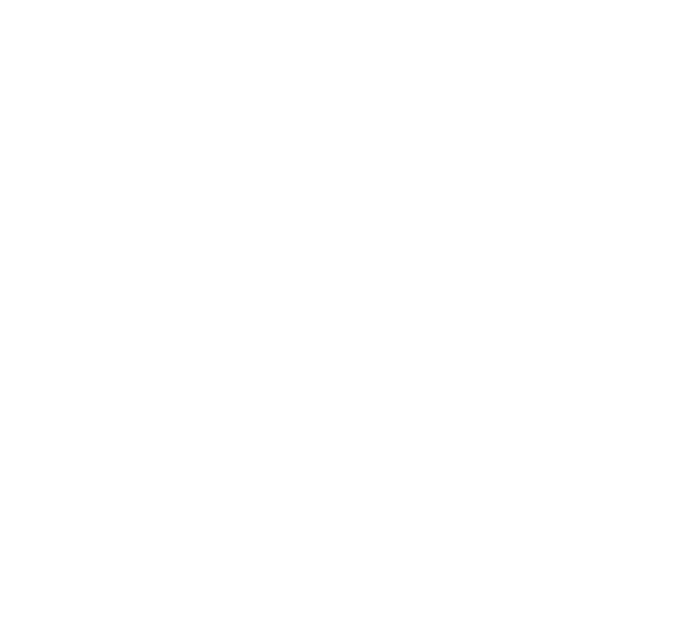
\includegraphics[scale=0.2]{Pictures/logo}
\end{center}
Industrial Engineering and Operations Research\\ Indian Institute of Technology Bombay}
\date{\today}
\begin{document}
% slide #1
\begin{frame}
% Cover slide
\titlepage
\end{frame}
% slide #2
\begin{frame}[t,allowframebreaks]
\frametitle{Overview}
\tableofcontents
%[pausesections]
\end{frame}
%--------------------------------------------------------
\section{Introduction}

%\subsection{Classical Multi-armed bandit problem}
\begin{frame}{Classical Multi-armed bandit problem}
\begin{itemize}
%\item We model the demand to change abruptly overtime
\item Gambler needs to decide each arm to play at each time instant
\item Each machine has different reward distribution unknown to the gambler
\item  Objective of the gambler is to maximize his total reward
\end{itemize}
%\begin{figure}
%\caption{Multi-armed bandit problem}
%\includegraphics[width=0.3\linewidth]{Pictures/one_arm_bandit_2}
%\color{Blue}Image courtesy - compare hatke}
%\floatfoot{Image courtesy - compare hatke}
%\caption{\textit{Image courtesy-Microsoft Research}}
%\end{figure}
\end{frame}
%---------------------------------------------------------
\section{Framework for correlated and stationary bandits}
\begin{frame}{Our Variant of the Multi-armed bandit problem}
\begin{itemize}
%\item We model the demand to change abruptly overtime
\item Set of bandit arms $N \equiv \{1,2...n\}$ have a corresponding feature $p_i$
\item Expected reward of arm $i$ is $\mu_i$
\item Reward of arm $i$ at time $t$, $$X_i(t)=p_i\times D(p_i,t)$$
\item $D(p_i,t)$ is a function of $p_i$ and time $t$ unknown to the user
\item $D(p_i,t)$ leads to a non-stationary bandit problem with dependent arms
\end{itemize} 
\end{frame}

\begin{frame}{Reward Structure of arms}

$$D(p_i,t)=N(1-F(p_i,t))+ \epsilon(t)$$
Hence, $\mu_i(t)=p_iN(1-F(p_i,t).$
\begin{itemize}
\item $N$ is a constant which remains same across all the arms
\item $\epsilon(t)$ corresponds to a residual error term ,
\begin{itemize}
\item $\epsilon(t)$ has mean $0$ 	
\item  $\epsilon(t)$ is i.i.d across time periods as well as arms
\end{itemize}




\end{itemize}





\end{frame}
\begin{frame}{Reward Structure of arms}
\begin{itemize}
\item $F(p,t )$ is given as follows
$$F(p,t) = 0\text{\ \ \ \ \ \ \ \    }\forall p \leq 0  $$
$$F(p,t) = \frac{p}{b(t)} \text{\ \ \ \ \ \ \ \    }\forall  0 \leq p \leq b(t)  $$
$$F(p,t) = 1 \text{\ \ \ \ \ \ \ \    } \forall   p \geq b(t)  $$
\item Non-stationarity arises as, $b(t)$ changes in a piece-wise constant manner at unknown time points (break points)

\item Assumption $0 \leq  p_i \leq b(t) \text{\ \ \ \ \ \ \ \    }  \forall p_i  \in \mathcal{P} \text{\ \ \ \ \ \ \ \    } \forall t$


\end{itemize}
\end{frame}

\begin{frame}{Regression based sliding window approach}
\begin{itemize}
\item To account for non-stationarity only the latest $\tau$ readings are considered
\item Parameters $N, b(t)$ are same across all n-arms
\item Estimate the rewards for all the arms by estimating the parameters as follows,
$$(\bar{N_t},\bar{b_t}(t))=  argmin_{N,b} \sum_{s=max(t-\tau,0)+1}^{t} (d(p_{I(s)},s)- N(1-\frac{p_{I(s)}}{b(t)}))^2 $$
$ \bar{N_t}$,$\bar{b_t}(t)$ denote the estimates of $N$ and $b(t)$ at time $t$\\
$d(p_{I(s)},s)$ represents the demand obtained at time $s$\\
$I(s)$ represents the arm played at time $s$
\end{itemize}
\end{frame}


\section{Greedy Algorithm}
\begin{frame}{Greedy Algorithm}
\begin{itemize}
\item No padding function
\item Plays the arm which has highest reward estimate 
%\item Used as a benchmark to compare other algorithm
\item Does not need the error term $\epsilon(t)$ to be truncated normal
\end{itemize}
\end{frame}

\begin{frame}{Greedy Algorithm}
\begin{algorithm}[H]
 \begin{footnotesize}
 
 

%\caption{Greedy algorithm}
\label{algo_Greedy}
\textbf{INITIALIZATION}:Play any two distinct arms in first two time periods\;
%\hspace{8cm} $t=2$}\;
 \For{ $t\leq T$}{
 \If {all observations in the window are from one particular arm then}{
 play any other arm randomly}
 \Else{
$
\bar{N_t},\bar{b_t}(t) = argmin_{N,b} \sum_{s=max(t-\tau,0)+1}^{min(t,\tau)} (d(p_{I(s)},s)- N(1-\frac{p_{I(s)}}{b(t)})^2 
$\\
 \textbf{Determine}(reward estimate $\bar{x_i}(t)$)\\
 \For{each arm $i$ do}{
$\bar{x_i}(t) = p_i \times \tilde{N}(1-\frac{p_i}{\tilde{b(t)}})$\;
} Play the arm which has maximum $\bar{x_i}(t)$\;

 } $t=t+1$\;}
 %\caption{Greedy algorithm}
 \end{footnotesize}
\end{algorithm}
\end{frame}



\subsection{Analysis of greedy algorithm}
\begin{frame}
\begin{footnotesize}
\begin{theorem}[Greedy algorithm worst case bounds]
\label{Greedy}
The Expected number of times a non optimal arm $i \in \mathcal{N}$ is played, when the Greedy algorithm is applied on $k$ bandit arms, fixed time horizon $T$ with a sliding window of length $\tau$ is bounded as follows :
\begin{multline*}E[\tilde{N_T}(i)] \leq 1+min_{m_1 \in \{1,..,\tau-2\}}\big[m_1+\sum_{t=3}^{\tau}2\times E_{\chi^2(t-2)}\big(\frac{\alpha_{maxN}(\sigma^2\times\chi^2(t-2),m_1)}{2}\big)\big]\\
+min_{m_2 \in \{1,..,\tau-1\}}\big[( \lceil{\frac{T}{\tau}}\rceil-1)m_2
+2\times(T-\tau) \times E_{\chi^2(\tau-2)}\big(\frac{\alpha_{maxN}(\sigma^2\times\chi^2(\tau-2),m_2)}{2}\big)\big]+\gamma_T\tau
\end{multline*}
where $\gamma_T$ are the number of breakpoints, $\chi^2(\tau-2)$ is chi-square distribution with $\tau-2$ degrees of freedom and \begin{multline*}\alpha_{max}(\sigma^2\times\chi^2(\tau-2),m)= 2\times P(t(RV)_{\tau-2} \geq \frac{\Delta\mu_T(i)}{2\times p_i \times \sqrt\frac{\sigma^2\times\chi^2(\tau-2)}{\tau-2} \times \sqrt{\frac{1}{\tau}+\frac{1}{m}}}  ).
\end{multline*} (here $t(RV)_{\tau-2}$ is a $t$ random variable with $\tau-2$ degrees of freedom) and $\Delta \mu_i(T)=min_{t \in \{1,..T\}}(\mu_{i*}(t)-\mu_i(t):i \neq i^*)$ .
\end{theorem}
\end{footnotesize}
\end{frame}
\begin{frame}{Interpretation of the upper bound}
\begin{itemize}


\item Bound can be viewed as a sum of stationary and non-stationary part

\item Non-Stationary Part
\begin{itemize}
\item  At most $\gamma_T\tau$ decision points contain data from before and after the breakpoint
\item $\gamma_T\tau$ is used to bound this part

\end{itemize}

\end{itemize}


\end{frame}

\begin{frame}{Interpretation of the upper bound}
\begin{itemize}
\item Stationary Part
\begin{itemize}
\item  1 is used to upper bound the number of times arm $i$ is played in first two time periods
\item  $
min_{m_1 \in \{1,..,\tau-2\}}\big[m_1+ \sum_{t=3}^{\tau}2\times E_{\chi^2(t-2)}\big(\frac{\alpha_{maxN}(\sigma^2\times\chi^2(t-2),m_1)}{2}\big)\big]
$
is an upper bound  from the time period $t=3$ to $t=\tau$
\item The third term,
$
 min_{m_2 \in \{1,..,\tau-1\}}\big[( \lceil{\frac{T}{\tau}}\rceil-1)m_2
+2\times(T-\tau)\times E_{\chi^2(\tau-2)}\big(\frac{\alpha_{maxN}(\sigma^2\times\chi^2(\tau-2),m_2)}{2}\big)\big]
$
upper bounds  from the time period $t=\tau+1$ to $t=T$ 
\item second and third term monotonically increase with decrease in $\Delta \mu_i(T)$ \\
$\Delta \mu_i(T)=min_{t \in \{1,..T\}}(\mu_{i*}(t)-\mu_i(t):i \neq i^*)$
\end{itemize}
\end{itemize}
\end{frame}

\begin{frame}{Bounds for the stationary case}
With length of window $\tau$ as $t$
\begin{multline*}
E[\tilde{N_T}(i)] \leq 1\\+min_{m_1 \in \{1,..,T-2\}}\big[m_1+\sum_{t=3}^{T}2\times E_{\chi^2(t-2)}\big(\frac{\alpha_{maxN}(\sigma^2\times\chi^2(t-2),m_1)}{2}\big)\big]
\end{multline*}
No terms of the form $kT$
\end{frame}
\subsection{Illustration of theoretical upper bounds}
\begin{frame}{Problem setting}
\begin{itemize}
\item Time horizon T=$130$
\item Arm set $\mathcal{N} \equiv \{ 1,2,3 \}$,  Feature set $\mathcal{P} \equiv {\{ 2, 3, 4 \}}$
\item $b(t)$ varies over time as follows
\begin{itemize}
\item $b(t)=5.5\quad \forall t \leq 40 $
\item $b(t)=4.5\quad \forall t \geq 40\quad and\quad t \leq 90$
\item $b(t)=9.0\quad \forall t \geq 90$
\end{itemize}
\item $N = 800$,$\epsilon(t)$ = $N(0,10^2)$ 
\item Length of sliding window $\tau = 20.$
\item Expected Reward
\begin{center}
\begin{tabular}{ |c|c|c|c| } 
 \hline
$\mu_i$ &$t \leq 40$  &  $40 \leq t \leq 90$ & $t \geq 90$ \\ 
\hline
 $\mu_1$ & 1018.18 &888.88 & 1244.44\\ 
 \hline
 $\mu_2$ & 1090.9090 &800&1600\\ 
 \hline
 $\mu_3$ & 1090.9090&355.56&1777.77\\
 \hline
\end{tabular}
\end{center}
\end{itemize}
\end{frame}

\begin{frame}{Input parameters for computation of upper bound }
\begin{enumerate}
\item Common parameters for all arms
\begin{enumerate}
\item Number of arms, $3$
\item Time horizon, $T=130$
\item Number of breakpoints, $\gamma_T=2$
\item $\sigma^2=10^2$
\end{enumerate}
\item Parameters specific to the arms
\begin{center}
\begin{tabular}{ |c|c|c|c| } 
 \hline
Parameters & Arm 1  &  Arm 2 & Arm 3 \\ 
\hline
 $p_i$ & $2$ & $3$ & $4$\\ 
 \hline
 $\Delta\mu_1$ & $72.729$ & $88.85$ & $218.182$\\ 
 \hline
\end{tabular}
\end{center}
\end{enumerate}
\end{frame}


\section{Bibliography}
\begin{frame}[t,allowframebreaks]
\frametitle{Bibliography}
\bibliography{Bibliography}
\end{frame}

\section{~}
\begin{frame}
%\begin{block}{}
\begin{center}
\Huge
Thank You!!!
\end{center}
%\end{block}
\end{frame}
\section*{Backup slides}
\begin{frame}

\begin{footnotesize}


\begin{theorem}[Greedy algorithm worst case bounds]
The Expected number of times a non optimal arm $i$ is played, when the Greedy algorithm is applied on $k$ bandit arms, fixed time horizon $T$ with a sliding window of length $\tau$ is bounded as follows :
\begin{multline*}E[\tilde{N_T}(i)] \leq \tau-1+\gamma_T\tau\\
+min_{m \in \{1,..,\tau-1\}}\big[( \lceil{\frac{T}{\tau}}\rceil-1)m\\
+2\times(T-\tau)\times E_{\chi^2(\tau-2)}\big(\frac{\alpha_{maxN}(\sigma^2\times\chi^2(\tau-2),m)}{2}\big)\big]
\end{multline*}
where $\gamma_T$ are the number of breakpoints and $$\alpha_{max}(\sigma^2\times\chi^2(\tau-2),m)= 2\times P(t(RV)_{\tau-2} \geq \frac{\Delta\mu_T(i)}{2\times p_i \times \sqrt\frac{\sigma^2\times\chi^2(\tau-2)}{\tau-2} \times \sqrt{\frac{1}{\tau}+\frac{1}{m}}}  ).$$ Also $\Delta \mu_i(T)=min_{t \in \{1,..T\}}(\mu_{i*}(t)-\mu_i(t):i \neq i^*)$ .
\end{theorem}
\end{footnotesize}
\end{frame}

\begin{frame}[t,allowframebreaks]

\begin{enumerate}

\item Number of times a non-optimal arm $i$ is played can be divided as follows:
\begin{align*}
\tilde{N_T}(i)=\sum_{t=1}^{2}1_{\{I(t)=i\neq i^*_t\}}+\sum_{t=3}^{\tau}1_{\{I(t)=i\neq i^*_t\}}+\sum_{t=\tau+1}^{T}1_{\{I(t)=i\neq i^*_t\}}\\
\tilde{N_T}(i)\leq 1+(\tau-2)+\sum_{t=\tau+1}^{T}1_{\{I(t)=i\neq i^*_t\}}\\
\end{align*}
(Since any two arms are played in the first two time periods)\\
Recollect that $I(t)$ represents the arm played at time $t$. Also $i^*_t$ represents the optimal arm at time $t$.
\\Now,
\begin{multline*}
\sum_{t=\tau+1}^{T}1_{\{I(t)=i\neq i^*_t\}}=\sum_{t=\tau+1}^{T}1_{\{I(t)=i\neq i^*_t,n_i(t,\tau)\leq m\}}
\\+\sum_{t=\tau+1}^{T}1_{\{I(t)=i\neq i^*_t,n_i(t,\tau)> m\}}
\end{multline*}
Here $n_i(t,\tau)$ is the number of times the arm has been played in the last $\tau$ periods, where for $t>\tau$
$$n_i(t,\tau) = \sum_{s=(t-\tau+1)}^{t}\{I(s)=i\}$$
for $t\leq \tau $,
$$n_i(t,\tau) = \sum_{s=1}^{t}\{I(s)=i\}$$

\begin{multline}
\label{eq1_1}
\therefore \tilde{N_T}(i)=\tau-1+\sum_{t=\tau+1}^{T}1_{\{I(t)=i\neq i^*_t, n_i(t,\tau)\leq m\}}
\\+\sum_{t=\tau+1}^{T}1_{\{I(t)=i\neq i^*_t, n_i(t,\tau)> m\}}
\end{multline}
\item Using  lemma \ref{lem_2} the first term in the right hand side of inequality \ref{eq1_1} can be bounded as follows

\begin{equation}\label{eq3_1}
\therefore \sum_{t=\tau+1}^{T}1_{\{I(t)=i\neq i^*_t, n_i(t,\tau)\leq  m)\}} \leq ( \lceil{\frac{T}{\tau}}\rceil-1)m
\end{equation}

%\textbf{from lemma 25 in non stationary bandit paper}

\item The second term in the right hand side of inequality \ref{eq1_1} can be bounded as follows
\begin{equation}
\label{eq4_1_g}
\sum_{t=\tau+1}^{T}1_{\{I(t)=i\neq i^*_t, n_i(t,\tau)> m\}} \leq \gamma_T\tau + \sum_{t\in \mathbb{T}(\tau)}1_{\{I(t)=i\neq i^*_t, n_i(t,\tau)> m\}}
\end{equation}
where ,\\
$\mathbb{T}(\tau)$ is a set of indices such that $t \in \{\tau,...T\}$ has $\mu_s(j)=\mu_t(j)$ \\  $\forall t- \tau \leq s \leq t$

\begin{itemize}
\item Now $\{I(t)=i\neq i^*_t, n_i(t,\tau)> m\}$ can be written as a subset of following events from lemma \ref{lem_1}
\begin{multline}
%\label{eq5}
\{I(t)=i\neq i^*_t, n_i(t,\tau)> m\} \subset \\
\{\bar{x_i}(t) \geq \bar{x_i^*}(t), n_i(t,\tau)> m\}\\
 \subset \{ \bar{x_i}(t) \geq \mu_t(i) +\frac{\mu_t(i^*)-\mu_t(i)}{2}, n_i(t,\tau)> m\}
\\ \cup \{\bar{x_i^*}(t) \leq \mu_t(i)- \frac{\mu_t(i^*)-\mu_t(i)}{2}, n_i(t,\tau)> m\}
\end{multline}
\\
But $$\{ \bar{x_i}(t) \geq \mu_t(i) +\frac{\mu_t(i^*)-\mu_t(i)}{2}\} \subset \{ \bar{x_i}(t) \geq \mu_t(i) +\frac{\Delta\mu_T(i)}{2}\}$$
and
$$\{\bar{x_i^*}(t) \leq \mu_t(i)- \frac{\mu_t(i^*)-\mu_t(i)}{2}\} \subset \{\bar{x_i^*}(t) \leq \mu_t(i)- \frac{\Delta\mu_T(i)}{2}\} $$
(recollect that $\Delta \mu_i(T)=min_{t \in \{1,..T\}}(\mu_{i*}(t)-\mu_i(t):i \neq i^*)$).\\
Hence,
\begin{multline}
\label{eq5_1}
\{I(t)=i\neq i^*_t, n_i(t,\tau)> m\} \subset \\
\{\bar{x_i}(t) \geq \bar{x_i^*}(t), n_i(t,\tau)> m\}\\
 \subset \{ \bar{x_i}(t) \geq \mu_t(i) +\frac{\Delta\mu_T(i)}{2}, n_i(t,\tau)> m\}
\\ \cup \{ \bar{x_i^*}(t) \leq \mu_t(i)-\frac{\Delta\mu_T(i)}{2}, n_i(t,\tau)> m\}
\end{multline}
 \item
We know that $\epsilon(t)$ is normal random variable. The sum of squared error ($sse_N$)  for normal random variable is defined as follows,
\begin{equation}
\begin{split}
sse_N:=\sum_{t-\tau+1}^{t}(D(p_{I(s)},s)-\bar{N}(1-\frac{p_{I(s)}}{\bar{b}(t)}))^2 
\end{split}
\end{equation}
\item
The mean square error mse is defined as follows,
$$mse:=\sqrt\frac{sse_N}{\tau-2}$$
 \item Now we interpret $\frac{\Delta\mu_T(i)}{2}$  as the confidence interval for the normal distribution. 
 $$\frac{\Delta\mu_i(T)}{2} = p_i\times t_{\frac{\alpha}{2},min(t-2,\tau-2)}\times mse \times \sqrt{\frac{1}{min(t,\tau)}+\frac{(p_i-\bar{p_{I(s)}})^2}{\sum_{s=t-\tau+1}^{t}(p_i-\bar{p_{I(s)}})^2}}$$
 
(Recollect that $p_I$ $(t,\tau )$ is the vector of all possible prices played in last $\tau $ periods. Hence
$$p_I(t,\tau) = (p_{I(t-\tau +1)},....p_{I(t)})$$
and $\bar{p_I} (t)$ is the mean of all the prices in $p_I (t)$.)


Since $ n_i(t,\tau) \geq m$,\\
we have 
\begin{multline}
\label{assmp_1}
\frac{\Delta\mu_i(T)}{2} \leq p_i\times t_{\frac{\alpha}{2},min(t-2,\tau-2)}\times mse \times \sqrt{\frac{1}{min(t,\tau)}+\frac{1}{m}}
\end{multline}
\item
Since $t\geq \tau$ we have
$$\therefore t_{\frac{\alpha}{2},\tau-2} \geq \frac{\Delta\mu_i(T)}{2\times p_i \times mse \times \sqrt{\frac{1}{\tau}+\frac{1}{m}}} $$


\begin{multline}\label{dagger}
\frac{\alpha}{2} = P(t(RV)_{\tau-2}\geq t_{\frac{\alpha}{2},\tau-2} )\\
\leq  P(t(RV)_{\tau-2} \geq \frac{\Delta\mu_i(T)}{2\times p_i \times \sqrt\frac{sse_N}{\tau-2} \times \sqrt{\frac{1}{\tau}+\frac{1}{m}}}  )	
\end{multline}
Let us denote the right hand side as, 

\begin{equation}\label{definition} \alpha_{max}(sse_N,m)= 2\times P(t(RV)_{\tau-2} \geq \frac{\Delta\mu_i(T)}{2\times p_i \times \sqrt{\frac{sse_N}{\tau-2}} \times \sqrt{\frac{1}{\tau}+\frac{1}{m}}}  )
\end{equation}


where $t(RV)_{\tau-2}$ is a random variable following $t$ distribution with $\tau-2$ degrees of freedom.





 



\item
Now,
\begin{multline}
P\{\bar{x_i}(t) \geq \mu_t(i) +\frac{\Delta\mu_i(T)}{2}, n_i(t,\tau)> m\} \\ 
=\int_{x=0}^{\infty}P\{\{\bar{x_i}(t) \geq \mu_t(i) +\frac{\Delta\mu_i(T)}{2}, n_i(t,\tau)> m\}|\{\frac{sse_N}{\sigma^2 }= x\}\}f_{\frac{sse_N}{\sigma^2  }}(x)dx\\
(\text{By conditioning on the value of } \frac{sse_N}{\sigma^2 }))\\
=\int_{x=0}^{\infty}P\{\bar{x_i}(t) \geq \mu_t(i) +\frac{\Delta\mu_i(T)}{2}, n_i(t,\tau)> m\}|\{\chi^2(\tau-2)= x\}\}f_{\chi^2(\tau-2)}(x)dx\\
(\text{We know that when error term is }N(0,\sigma^2), \frac{sse_N}{\sigma^2} \text{in that case has the} \\ \chi^2(\tau-2) \text{distribution.}\text{(See Klimov \cite{klimov1986probability})})\\
\leq \int_{x=0}^{\infty}P(t(RV)_{\tau-2}\geq \frac{\Delta\mu_i(T)}{2\times p_i \times \sqrt\frac{\sigma^2\times x}{\tau-2} \times \sqrt{\frac{1}{\tau}+\frac{1}{m}}}  )\times f_{\chi^2(\tau-2)}(x)dx \\
(\text{Since we interpret}  \Delta\mu_i(T)  \text{ as the confidence interval }  and \text{ by using inequality \ref{dagger}})\\
= E_{\chi^2(\tau-2)}(\big(\frac{\alpha_{maxN}(\sigma^2\times\chi^2(\tau-2),m)}{2}\big)\\
(\text{By defiition of} \alpha_{max}(sse_{N},m) \text{ see equation \ref{definition} })
\end{multline}
Hence,
\begin{multline}\label{eq_11_1}
P\{\bar{x_i}(t) \geq \mu_t(i) +\frac{\Delta\mu_i(T)}{2}, n_i(t,\tau)> m\} \\ \leq E_{\chi^2(\tau-2)}\big(\frac{\alpha_{maxN}(\sigma^2\times\chi^2(\tau-2),m)}{2}\big)
\end{multline}
Similarly,
\begin{multline}
\label{eq_12_1}
P\{\bar{x_i}(t) \leq \mu_t(i)-\frac{\Delta\mu_i(T)}{2}, n_i(t,\tau)> m\} \\ \leq E_{\chi^2(\tau-2)}\big(\frac{\alpha_{maxN}(\sigma^2\times\chi^2(\tau-2),m)}{2}\big)
\end{multline}

From equations \ref{eq_11_1},\ref{eq_12_1}, when $t \in \mathbb{T}(\tau)$
\begin{equation}\label{eq13}
\therefore
P\{I(t)=i\neq i^*_t, n_i(t,\tau)> m\} \leq 2 \times E_{\chi^2(\tau-2}(\big(\frac{\alpha_{maxN}(\sigma^2\times\chi^2(\tau-2),m)}{2}\big)
\end{equation}
From equation \ref{eq4_1_g} we have
\begin{multline}
\label{12_1_1}
\mathbb{E}(\sum_{t=\tau+1}^{T}1_{\{I(t)=i\neq i^*_t, n_i(t,\tau)> m\}}) \leq \gamma_T\tau + \mathbb{E}(\sum_{t\in \mathbb{T}(\tau)}1_{\{I(t)=i\neq i^*_t, n_i(t,\tau)> m\}})\\
\leq \gamma_T\tau + (T-\tau)\times 2 \times E_{\chi^2(\tau-2}\big(\frac{\alpha_{maxN}(\sigma^2\times\chi^2(\tau-2),m)}{2}\big)
\end{multline}
(Since $|\mathbb{T(\tau)}|\leq (T-\tau)$ )
\end{itemize}
\item From equation \ref{eq1_1},\ref{eq3_1},\ref{12_1_1} we have \\

\begin{multline}
E[\tilde{N_T}(i)] \leq \tau-1+( \lceil{\frac{T}{\tau}}\rceil-1)m+\gamma_T\tau\\+2\times(T-\tau)\times E_{\chi^2(\tau-2)}\big(\frac{\alpha_{maxN}(\sigma^2\times\chi^2(\tau-2),m)}{2}\big)
\end{multline}

\end{enumerate}
But this holds for every positive integer $m$. Note that the bound becomes trivial if $m \geq \tau$. 
Hence we have
\begin{multline}
E[\tilde{N_T}(i)] \leq min_{m \in \{1,..,\tau-1\}}(\tau-1+( \lceil{\frac{T}{\tau}}\rceil-1)m\\+\gamma_T\tau+2\times(T-\tau)\times E_{\chi^2(\tau-2)}\big(\frac{\alpha_{maxN}(\sigma^2\times\chi^2(\tau-2),m)}{2}\big)
\end{multline}




\end{frame}

\begin{frame}
\begin{footnotesize}

\begin{theorem}[Worst case bounds for Regression Based UCB algorithm when the error term is normal]
\label{thm:rucb}
The Expected number of times a non optimal arm $i$ is played, when the Regression Based UCB algorithm is applied on $k$ bandit arms, fixed time horizon $T$ with a sliding window of length $\tau$ and level of significance $\alpha=\frac{1}{\tau^4}$   is bounded as follows :
\begin{multline*}E[\tilde{N_T}(i)] \leq \tau-1+2\times\frac{T-\tau}{\tau^4}+\gamma_T\tau\\+ min_{m \in \{1,..,\tau-1\} }[(T-\tau)\times P\{\frac{\Delta \mu_i(T)^2}{\sigma^2 \times B(i,\tau)^2 \times (\frac{1}{\tau}+\frac{1}{m})} \leq \chi^2(\tau-2)\}\\+( \lceil{\frac{T}{\tau}}\rceil-1)m]
\end{multline*}
Here $\gamma_T$ are the number of breakpoints, $B(i,\tau)=(2 \times p_i\times t_{\frac{\alpha}{2},min(t-2,\tau-2)}\times \sqrt{\frac{1}{\tau-2}} )$ and $\Delta \mu_i(T)=min_{t \in \{1,..T\}}(\mu_{i*}(t)-\mu_i(t):i \neq i^*)$
\end{theorem}

\end{footnotesize}
\end{frame}
\begin{frame}[t,allowframebreaks]
\begin{enumerate}
\item Number of times a non-optimal arm $i$ is played can be divided as follows:
\begin{align*}
\tilde{N_T}(i)=\sum_{t=1}^{2}1_{\{I(t)=i\neq i^*_t\}}+\sum_{t=3}^{\tau}1_{\{I(t)=i\neq i^*_t\}}+\sum_{t=\tau+1}^{T}1_{\{I(t)=i\neq i^*_t\}}\\
\tilde{N_T}(i)\leq 1+(\tau-2)+\sum_{t=\tau+1}^{T}1_{\{I(t)=i\neq i^*_t\}}\\
\end{align*}
(Since any two arms are played in the first two time periods)\\
Recollect that $I(t)$ represents the arm played at time $t$. Also $i^*_t$ represents the optimal arm at time $t$.
\\Now,
\begin{multline*}
\sum_{t=\tau+1}^{T}1_{\{I(t)=i\neq i^*_t\}}=\sum_{t=\tau+1}^{T}1_{\{I(t)=i\neq i^*_t,n_i(t,\tau)\leq m\}}
\\+\sum_{t=\tau+1}^{T}1_{\{I(t)=i\neq i^*_t,n_i(t,\tau)> m\}}
\end{multline*}
Here $n_i(t,\tau)$ is the number of times the arm has been played in the last $\tau$ periods, where for $t>\tau$
$$n_i(t,\tau) = \sum_{s=(t-\tau+1)}^{t}\{I(s)=i\}$$
for $t\leq \tau $,
$$n_i(t,\tau) = \sum_{s=1}^{t}\{I(s)=i\}$$

\begin{multline}
\label{eq1_1_1}
\therefore \tilde{N_T}(i)=\tau-1+\sum_{t=\tau+1}^{T}1_{\{I(t)=i\neq i^*_t, n_i(t,\tau)\leq m\}}
\\+\sum_{t=\tau+1}^{T}1_{\{I(t)=i\neq i^*_t, n_i(t,\tau)> m\}}
\end{multline}
\item Using  lemma \ref{lem_2} the first term in the right hand side of inequality \ref{eq1_1_1} can be bounded as follows

\begin{equation}\label{eq3_1_1}
\therefore \sum_{t=\tau+1}^{T}1_{\{I(t)=i\neq i^*_t, n_i(t,\tau)\leq  m)\}} \leq ( \lceil{\frac{T}{\tau}}\rceil-1)m
\end{equation}


\item The second term in the right hand side of equation \ref{eq1_1_1} can be bounded as follows.
\begin{equation}
\label{eq4_1}
\sum_{t=\tau+1}^{T}1_{\{I(t)=i\neq i^*_t,n_i(t,\tau)> m\}} \leq \gamma_T\tau + \sum_{t\in \mathbb{T}(\tau)}1_{\{I(t)=i\neq i^*_t,n_i(t,\tau)> m\}}
\end{equation}
\\($\mathbb{T}(\tau)$ is a set of indices such that $t \in \{\tau+1,...T\}$ has $\mu_s(j)=\mu_t(j)$ \\  $\forall t-\tau \leq s \leq t$)
\begin{itemize}
\item Now $\{I(t)=i\neq i^*_t,n_i(t,\tau)> m \}$ can written as a subset of following events by using lemma \ref{lem_1}.
\begin{multline}
\label{eq5}
\{I(t)=i\neq i^*_t,n_i(t,\tau)> m\}\subset \\
\{\bar{x_i}(t)+ PF_i(t,\tau,p_I(t,\tau)) \geq \bar{x_{i^*}}(\tau,i^*)+ PF_{i^*}(t,\tau,p_I(t,\tau)),n_i(t,\tau)> m \}\\
\subset \{ \bar{x_i}(t) \geq \mu_t(i) + PF_{i}(t,\tau,p_I(t,\tau))\}  \cup \{\bar{x_{i^*}}(t) \leq \mu_t(i) - PF_{i^*}(\tau,i^*)\}\\
\cup \{\mu_t(i^*)-\mu_t(i) \leq 2PF_{i}(\tau,i),n_i(t,\tau)> m\}
\end{multline}


\item
Padding function for arm $i$=$PF_{i}(t,\tau,p_I(t,\tau))$

\begin{multline}
PF_{i}(t,\tau,p_I(t,\tau))\\= p_i\times t_{\frac{\alpha}{2},min(t-2,\tau-2)}\times mse \times \sqrt{\frac{1}{min(t,\tau)}+\frac{(p_i-\bar{p_{I(s)}})^2}{\sum_{s=t-\tau+1}^{t}(p_i-\bar{p_{I(s)}})^2}}
\end{multline}

(Recollect that $p_I$ $(t,\tau )$ is the vector of all possible prices played in last $\tau $ periods. Hence
$$p_I(t,\tau) = (p_{I(t-\tau +1)},....p_{I(t)})$$
and $\bar{p_I} (t)$ is the mean of all the prices in $p_I (t)$. )\\
Since $n_i(t,\tau) \geq m$
$$\sum_{s=t-\tau+1}^{t}(p_i-\bar{p_{I(s)}})^2  \geq m(p_i-\bar{p_{I(s)}})^2$$
$$\therefore PF_{i}(t,\tau,p_I(t,\tau)) \leq p_i\times t_{\frac{\alpha}{2},min(t-2,\tau-2)}\times mse \times \sqrt{\frac{1}{min(t,\tau)}+\frac{1}{m}}$$
when $t > \tau$
\begin{equation}
\label{star}
PF_{i}(t,\tau,p_I(t,\tau)) \leq p_i\times t_{\frac{\alpha}{2},\tau-2}\times mse \times \sqrt{\frac{1}{\tau}+\frac{1}{m}}
\end{equation}
\item
We know that $\epsilon(t)$ is normal random variable. The sum of squared error is defined as
\begin{equation}
\begin{split}
sse_N := \sum_{t-\tau+1}^{t}(D(p_{I(s)},s)-\bar{N}(1-\frac{p_{I(s)}}{\bar{b}(t)}))^2 
\end{split}
\end{equation}

We know that when error term is $N(0,\sigma^2)$ , the sum of squared error in that case ($sse_N$) has the $\sigma^2\times\chi^2(\tau-2)$ distribution. See Klimov \cite{klimov1986probability} . \\
The mean square error $mse$ is defined as
$$mse:=\sqrt{\frac{sse_N}{\tau-2}}$$

Now when $t \in \mathbb{T}(\tau)$
\begin{multline}
\{\mu_t(i^*)-\mu_t(i) \leq 2PF_{i}(t,\tau,p_I(t,\tau)) ,n_i(t,\tau)> m\} \\ \subset \{\Delta \mu_i(T) \leq 2PF_{i}(t,\tau,p_I(t,\tau)) ,n_i(t,\tau)> m\} \\
\subset \{\Delta \mu_i(T) \leq 2 \times p_i\times t_{\frac{\alpha}{2},min(t-2,\tau-2)}\times mse \times \sqrt{\frac{1}{\tau}+\frac{1}{m}}\}\\ \text{(Because of equation \ref{star})} \\
\equiv \{\Delta \mu_i(T) \leq 2 \times p_i\times t_{\frac{\alpha}{2},min(t-2,\tau-2)}\times \sqrt{\frac{sse_N}{\tau-2}} \times \sqrt{\frac{1}{\tau}+\frac{1}{m}}\}
\end{multline}
(recollect that $\Delta \mu_i(T)=min_{t \in \{1,..T\}}(\mu_{i*}(t)-\mu_i(t):i \neq i^*)$)

As $B(i,\tau)=(2 \times p_i\times t_{\frac{\alpha}{2},min(t-2,\tau-2)}\times \sqrt{\frac{1}{\tau-2}} )$
\begin{multline}\{\Delta \mu_i(T) \leq 2 \times p_i\times t_{\frac{\alpha}{2},min(t-2,\tau-2)}\times \sqrt{\frac{sse_N}{\tau-2}} \times \sqrt{\frac{1}{\tau}+\frac{1}{m}}\} \\ \equiv \{{\Delta \mu_i(T)}^2 \leq B(i,\tau)^2 \times (\frac{1}{\tau}+\frac{1}{m})\times sse_N\}
\end{multline}
(Since everything is positive)


\begin{multline}\label{eq7}
\therefore P\{\mu_t(i^*)-\mu_t(i) \leq 2c_t(\tau,i)\} \\ \leq P\{\frac{\Delta \mu_i(T)^2}{B(i,\tau)^2 \times (\frac{1}{\tau}+\frac{1}{m})} \leq sse_N\}\\
\leq P\{\frac{\Delta \mu_i(T)^2}{B(i,\tau)^2 \times (\frac{1}{\tau}+\frac{1}{m})} \leq \sigma^2\times\chi^2(\tau-2)\}\\
\end{multline}
(See Klimov \cite{klimov1986probability} et al. )

\item

%We use the fact that truncated normal distribution for the same significance level would have a lower  confidence interval as compared to normal random variable. This is because variance of truncated normal random variable is lower than variance of normal variable.
\begin{multline}\label{eq8}
P\{ \bar{x_i}(t) \geq \mu_t(i) + PF_{i}(t,\tau,p_I(t,\tau)))\}  
\\=P\{ \bar{x_i}(t) \leq \mu_t(i) - PF_{i}(t,\tau,p_I(t,\tau))\}  = \frac{1}{\tau^4} 
\end{multline}
\text{(from the definition of confidence interval)}
\\Similarly,
\begin{multline}\label{eq9}
P\{\bar{x_{i^*}}(t) \leq \mu_t(i) - PF_{i^*}(t,\tau,p_I(t,\tau))\}
\\=P\{\mu_t(i)  \geq \bar{x_{i^*}}(t)+ PF_{i^*}(t,\tau,p_I(t,\tau)\} \leq \frac{1}{\tau^4} 
\end{multline}
\item 
From equation \ref{eq5} we have
\begin{multline}
P\{I(t)=i\neq i^*_t,n_i(t,\tau)> m\} \leq P\{ \bar{x_i}(t) \geq \mu_t(i) + PF_{i}(t,\tau,p_I(t,\tau)\}  
\\ + P\{\bar{x_{i^*}}(t) \leq \mu_t(i) - PF_{i^*}(t,\tau,p_I(t,\tau)\}
\\ + P\{\mu_t(i^*)-\mu_t(i) \leq 2PF_{i}(t,\tau,p_I(t,\tau),n_i(t,\tau)>m\}
\end{multline}
From equations \ref{eq7},\ref{eq8},\ref{eq9}, when $t \in \mathbb{T(\tau)}$
\begin{multline}\label{eq11}
\therefore
P\{I(t)=i\neq i^*_t,n_i(t,\tau)> m\} \leq \frac{2}{\tau^4}
\\ + P\{\frac{\Delta \mu_i(T)^2}{\sigma^2 \times B(i,\tau)^2 \times (\frac{1}{\tau}+\frac{1}{m})} \leq \chi^2(\tau-2)\}
\end{multline}
From equation \ref{eq4_1} we have
\begin{multline}
\label{12_1}
\mathbb{E}(\sum_{t=\tau+1}^{T}1_{\{I(t)=i\neq i^*_t,n_i(t,\tau)> m\}}) \leq \gamma_T\tau + \mathbb{E}(\sum_{t\in \mathbb{T}(\tau)}1_{\{I(t)=i\neq i^*_t,n_i(t,\tau)> m\}})\\
\end{multline}
\begin{multline}
\label{12}
\text{Now from equation \ref{eq11} we have                      }\\
\mathbb{E}(\sum_{t=\tau+1}^{T}1_{\{I(t)=i\neq i^*_t,n_i(t,\tau)> m\}}) \leq  \gamma_T\tau+\sum_{t\in \mathbb{T}}(\frac{2}{\tau^4}\\+ P\{\frac{\Delta \mu_i(T)^2}{\sigma^2 \times B(i,\tau)^2 \times (\frac{1}{\tau}+\frac{1}{m})} \leq \chi^2(\tau-2)\})
\end{multline}

\end{itemize}
\item From equation \ref{eq1_1_1}, \ref{eq3_1_1}, \ref{12} we have \\

\begin{multline}
E[\tilde{N_T}(i)] \leq 1 + max(\tau-k,0)+( \lceil{\frac{T}{\tau}}\rceil-1)m+\gamma_T\tau+2\times\frac{T-\tau}{\tau^4}\\+ (T-\tau)\times P\{\frac{\Delta \mu_i(T)^2}{\sigma^2 \times B(i,\tau)^2 \times (\frac{1}{\tau}+\frac{1}{m})} \leq \chi^2(\tau-2)\}
\end{multline}
\text{(Since $|\mathbb{T}(\tau)| \leq T-\tau$) }
\end{enumerate}
But this holds for every positive integer $m$. Note that the bound becomes trivial if $m \geq \tau$. 
Hence we have
\begin{multline}
E[\tilde{N_T}(i)] \leq min_{m \in \{1,..,\tau-1\}}(1 + max(\tau-k,0)+( \lceil{\frac{T}{\tau}}\rceil-1)m+\gamma_T\tau+2\times\frac{T-\tau}{\tau^4}\\+ (T-\tau)\times P\{\frac{\Delta \mu_i(T)^2}{\sigma^2 \times B(i,\tau)^2 \times (\frac{1}{\tau}+\frac{1}{m})} \leq \chi^2(\tau-2)\})
\end{multline}


\end{frame}
\begin{frame}[t,allowframebreaks]
\begin{lemma}\label{lem_2}
For an arm $i \in \mathbb{N}$ and for a sliding window length $\tau$ ,\begin{multline}\sum_{t=\tau+1}^{T}1_{\{I(t)=i, n_i(t,\tau) \leq m\}} \leq( \lceil{\frac{T}{\tau}}\rceil-\lfloor{\frac{\tau}{\tau}}\rfloor) m \\ \leq( \lceil{\frac{T}{\tau}}\rceil-1) m
\end{multline}
\end{lemma}
\end{frame}
\begin{frame}
\begin{tiny}




\begin{proof}
$$\sum_{t=\tau+1}^{T}1_{\{I(t)=i, n_i(t,\tau) \leq m\}} \leq \sum_{j=\lfloor{\frac{\tau}{\tau}}\rfloor+1}^{ \lceil{\frac{T}{\tau}}\rceil}\sum_{t=(j-1)\tau+1}^{j\tau}1_{\{I(t)=i, n_i(t,\tau) \leq m\}}$$ 

Now, $\sum_{t=(j-1)\tau+1}^{j\tau}1_{\{I(t)=i, n_i(t,\tau) \leq m\}}$ is non-zero if for some $t \in {(j-1)\tau+1,...,(j)\tau+1}$ , we have ${I(t)=i, n_i(t,\tau) \leq m}$ .\\ Let $t_j$ be the maximum time this happens in $j^{th}$ interval 
 $$\therefore t_j=max({t \in {(j-1)\tau+1,...,(j)\tau+1}:{I(t)=i, n_i(t,\tau) \leq m}})$$
\begin{multline*}\therefore \sum_{t=(j-1)\tau+1}^{j\tau}1_{\{I(t)=i, n_i(t,\tau) \leq m\}}\\
 = \sum_{t=(j-1)\tau+1}^{t_j}1_{\{I(t)=i,n_i(t,\tau) \leq m\}}\\
\leq \sum_{t=t_j-\tau+1}^{t_j}1_{\{I(t)=i,n_i(t,\tau) \leq m\}} \leq \sum_{t=t_j-\tau+1}^{t_j}1_{\{I(t)=i\}} = n_i(t,\tau) \leq m
\end{multline*}

\end{proof}
\end{tiny}
\end{frame}

\begin{frame}
\begin{lemma}\label{lem_1}
If $$D \cap A^c \cap B^c \subset C$$ than $$D \subset A \cup B \cup C$$
\end{lemma}
\end{frame}
\begin{frame}
\begin{footnotesize}


\begin{proof}
$$D \cap A^c \cap B^c \subset C$$ 
$$\therefore D \cap (A\cup B )^c\subset C$$ 
$$\therefore (D \cap (A\cup B )^c) \cup (A \cup B)\subset C\cup A \cup B$$ 
$$\therefore (D  \cup (A \cup B)) \cap ((A\cup B )^c \cup (A \cup B)) \subset C\cup A \cup B$$ 
$$\therefore D  \cup (A \cup B) \subset C\cup A \cup B$$ 
But
$$D \subset D  \cup (A \cup B)  $$
$$\therefore D  \subset C\cup A \cup B$$
\end{proof}
\end{footnotesize}
\end{frame}

\begin{frame}{Computation of expected regret}
\begin{itemize}
\item The computation of expected regret is done by averaging the number of times a each arm is played at each time period over $100$ replications
\item This value of fraction of times a each arm is played at each time period is multiplied by the regret associated with that arm at that time period
\item Summing over the value of regret of all arms at that time period we get the instantaneous value of regret at that time period
\item Summing over all such values upto that time period, we get the value of expected regret
\end{itemize}

\end{frame}
\end{document}

